% input files


% \begin{table}[h]
%     \centering
%     \caption{Дифференциальные уравнения}
%         \begin{tabular}{lll}
%     \toprule
%             Тип & Вид & Уязвимость \\
%     \midrule
%             \textbf{одн. ур.} &
%             $y' = f\left(\frac{y}{x}\right)$ &
%             $y = t(x) \cdot x$ \\
%             & $y' = f\left(\frac{a_1 x + b_1 y + c}{ax + by + c} \right)$ &
%             I. $z = ax + by + c$ \\
%             & & II. $O \to l_1 \cap l_2$\\
%             \multicolumn{3}{c}{Можно свести к одн. ур. заменой $y = z^m$} \\
%     \midrule
%             \textbf{лин. ур. I пор.} &
%             $y' + a(x) y = b(x)$ &
%             $y' + a(x) y = 0; \hspace{0.5cm} C \to C(x)$
%             \\
%             ур. Бернулли &
%             $y' + a(x)y = b(x) y^n, (n \neq 1)$ &
%             $/ y^n, \hspace{0.5cm} z = 1 / y^{n-1}$ \\
%             ур. Риккати &
%             $y' + a(x) y + b(x) y^2 = c(x)$ &
%             $\letus y_1(x) \in \text{Sol}$, \hspace{0.5cm} $y = y_1 + z$\\
%             \multicolumn{3}{r}{см. свободный член} \\
%     \bottomrule
%         \end{tabular}
%     \label{tab:1}
% \end{table}

 


% document's head
% \phantom{42}

\begin{center}
    \LARGE \textsc{Заметки курса <<Электричество и магнетизм>>}
\end{center}

\hrule

\phantom{42}

\begin{flushright}
    \begin{tabular}{rr}
    % written by:
        \textbf{Автор}: 
        & Хоружий Кирилл \\
        &\\
    % date:
        \textbf{От}: &
        \textit{\today}\\
    \end{tabular}
\end{flushright}

\thispagestyle{empty}
\tableofcontents
% \newpage


%%%%%%%%%%%%%%%%%%%%%%%%%%%%%%%%%%%%%%%%%%%%%%%%%%%%%%%%%%%%%%%%%%%%%%%%%%%%%%%%%%%
\setcounter{section}{1}
\addcontentsline{toc}{section}{Электрическое поле}
%%%%%%%%%%%%%%%%%%%%%%%%%%%%%%%%%%%%%%%%%%%%%%%%%%%%%%%%%%%%%%%%%%%%%%%%%%%%%%%%%%%

\sbsnum{1}{Электрические заряды и закон Кулона}
\section{Закон Кулона и теорема Гаусса}

Здесь попробуем индуктивно построить содержательную теорию, \textbf{начнём с двух эксперементальных фактов}, положенных в основу теории. Закона Кулона (сгсэ)
\begin{equation}
    \vc{F} = \frac{q_1 q_2 }{r^2} \frac{\vc{r}}{r},
\end{equation}
и, введя вектор напряженности электростатического поля $\vc{E} = \vc{F} / q$, принцип суперпозиции:
\begin{equation}
    \vc{E} = \sum \vc{E}_i.  
\end{equation}

\subsubsection*{Дипольный момент}
Простейшим примером системы зарядов является диполь $q_1 + q_2 = 0$, для которого введём $\vc{p}=q \vc{l}$:
$$
    \vc{E} = \frac{q}{r_1^2} \frac{\vc{r}_1}{r_1} - \frac{q}{r_1^2} \frac{\vc{r}_2}{r_2} 
    \hspace{0.5cm} \overset{l \ll r_2, r_1}{\underset{\Longrightarrow}{}} \hspace{0.5cm} 
    \vc{E} = \frac{3 (\vc{p} \cdot \vc{n}) \vc{n}}{r^3}  - \frac{\vc{p}}{r^3}
$$

Для заряженной нити верно, что
$$
    E = 2 \frac{\varkappa}{r}. 
$$



Теперь дойдём до двух теорем (кусочки уравнений Максвелла), описывающих электростатическое поле. 
\begin{to_thr}[теорема Гаусса]
    Для потока $\vc{E}$ через замкнутую поверхность $S$ верно, что
    \begin{equation}
        \oint_S E_n \d S =
        \oint_S (\vc{E} \d \vc{S}) 
        = 4 \pi q_{\textnormal{вн}}.
    \end{equation}
\end{to_thr}


\begin{proof}[$\triangle$]
\textcolor{grey}{
    \begin{minipage}[t]{0.9\textwidth}
        \begin{enumerate}[label = \Roman*.]
            \item Доказательство (из закона Кулона) для сферы вокруг точечного заряда очевидно. 
            \item Рассмотрим произвольную поверхность $\Omega$, содержащую заряд, и телесный угол в онной:
            $$
                E_n \d S = E \cos \alpha \d S = E \d S' 
            $$
            То есть поток через наклонную площадку равен потоку через тот же телесный угол через некоторую вспомогательную сферу. Так как $s_1 / s_2 = r_1^2 / r_2^2$ и $E_1 / E_2 = r_2^2/r_1^2$, получается интегрировать по $\Omega$ то же самое, что и интегрировать по выбранной хорошей сфере. 
            \item Рассмотрим теперь некоторую $\Omega$, не содержащую заряд. Посмотрим на телесный угол от $q$. По модулю потоки через них одинаковые, а знаки противоположны, следовательно вклада в поток через $\Omega$ нет.
            \item Для сложного распределения зарядов, по принципу суперпозиции верно, что
            $$
                \vc{E} = \sum_i \vc{E}_i
                \hspace{0.5cm} \Rightarrow \hspace{0.5cm} 
                \oint_S E_n \d S = \sum_i \oint_S \vc{E}_i \d S.
            $$
        \end{enumerate}
    \end{minipage}
}

\phantom{42}
\end{proof}



\newpage 

\sbsnum{2}{Электрическое поле и основная задача электростатики}
Вместо поиска $\vc{E}$ достаточно найти $\varphi$,
\begin{equation*}
    \left\{\begin{aligned}
        &\vc{E} = -\frac{1}{c}\frac{\partial \vc{A}}{\partial t} - \grad \varphi \\
        &\div \vc{E} = 4 \pi \rho \\
    \end{aligned}\right.
    \hspace{0.5cm} \Rightarrow \hspace{0.5cm} 
    \div \grad \varphi \equiv \Delta \varphi = 
    \left\{\begin{aligned}
        &- 4 \pi \rho &\text{ур. Пуассона} \\
        &\phantom{42} 0 &\text{ур. Лапласа}
    \end{aligned}\right.
\end{equation*}


Как может быть поставлена задача? Заданы граничные значения, найти распределения зарядов. Заданы заряды, найти распределения. Что-то задано, что-то не задано. Во всех трёх случаях \textbf{решение уравнения Пуассона единственно}. 


К слову, так как $\varphi = \varphi(\vc{r})$, а при $A_i = \const$ верно, что $\vc{E} = -\grad \varphi$, то электростатическое поле потенциально. Также это можно увидеть в работе ЭМ сил, при перемещении заряда по замкнутому контуру:
\begin{equation*}
    A_{\text{замкн}}/q = \oint_{(L)} \vc{E} \cdot \d \vc{l} = - \frac{1}{c} \frac{\partial }{\partial t} \int \vc{H} \cdot \d \vc{f} = 0.
\end{equation*}

\vspace{-10pt}

\subsubsection*{Разность потенциалов}

\begin{to_def} 
      Если на участке цепи не действуют сторонние силы, работа по перемещению включает только работу потенциального электрического поля и \textit{электрическое напряжение} $U_{AB}$ между $A$ и $B$ совпадает с разностью потенциалов $\varphi_A - \varphi_B = A^{\text{el}}_{AB}/q$. В общем случае $U_{AB} = \varphi_A - \varphi_B + \mathscr{E}_{AB}$.
\end{to_def}

\subsubsection*{Граничные условия на заряженной поверхности}

\vspace{-10pt}

\begin{minipage}[c]{0.45\textwidth}
\noindent
    По теореме Гаусса верно, что
    \begin{align*}
        E_{2n_2} \cancel{\Delta S} + E_{1n_1} \cancel{\Delta S} &= 4\pi\sigma \cancel{\Delta S}, \\
        E_{2n} - E_{1n} &= 4\pi\sigma
    \end{align*}
\noindent
    По теореме циркуляции верно, что
    \begin{align*}
        E_{2l} \cancel{\Delta} l - E_{1l} \cancel{\Delta} l &= 0 \\
        E_{2l} - E_{1l} &= 0.
    \end{align*}
\end{minipage}
\hfill
\begin{minipage}[c]{0.45\textwidth}
    \incfig{3}
\end{minipage}

\vspace{-10pt}

\subsubsection*{Проводники}

\begin{to_def}[пусть так]
    \textit{Проводник} -- костяк частиц, окруженных \textit{свободными} электронами, которые в пределах тела могут перемещаться на какие угодно
    расстояния. 
\end{to_def}

\vspace{-10pt}

\begin{minipage}[c]{0.55\textwidth}
    В частности, для проводников, верно, что
    \begin{align*}
        E_n &= 4 \pi \sigma \\
        E_\tau &= 0
    \end{align*}
\end{minipage}
\hfill
\begin{minipage}[c]{0.35\textwidth}
    \incfig{4}
\end{minipage}

Собственно, объёмных зарядов в проводнике нет, поверхностные есть и компенсируют внешнее поле. Аналогично работает решетка Фарадея, электростатическое поле не проникает в проводники.


\subsubsection*{Метод изображений}

Если существует некоторая эквипотенциальная поверхность разделяющая пространство на два полупространства, то можем считать что эта поверхность является проводящей. И наоборот, проводящую поверхность можно заменить, на системы зарядов в полупространстве, ей ограниченном, создающих эквипотенциальную поверхность.


\newpage 

\sbsnum{3}{Электрическое поле в веществе}
\subsection{Дифференциальная форма}

В линейной алгебре есть ковекторы, а вот в дифференциальной геометрии ковекторные поля суть дифференциальные 1-формы.

\begin{to_def} 
    \textit{Дифференциальная 1-форма} -- это  ковекторное поле.
\end{to_def}

\begin{to_def} 
    \textit{Дифференциал} функции $f$ от векторного поля $X$ это
    $
        d f (X) \overset{\mathrm{def}}{=}  X f.
    $
\end{to_def}

Что это нам даёт? Ну, во-первых, пусть $\set{x}{n}$ -- некоторые координаты. 
$$
    X = X^i \frac{\partial }{\partial x^i}.
$$
Тогда
$$
    df(X) = Xf = X^i \frac{\partial f}{\partial x^i}.
$$
Но, заметим, что $\frac{\partial }{\partial x^1}, \ldots, \frac{\partial }{\partial x^n}$ -- базис в каждой точке. Рассмотрим теперь $f = x^i$ и $X = \frac{\partial }{\partial x^j} $, тогда
\begin{equation}
    d x^i \left(\frac{\partial }{\partial x^j} \right)
    =
    \frac{\partial x^i}{\partial x^j} = \delta^i_j.
\end{equation}
Из этого следует, что $\set{dx}{n}$ -- двойственный к $\frac{\partial }{\partial x^1}, \ldots, \frac{\partial }{\partial x^n}$ базис в $V^*$.
Тогда в этом базисе
$$
    d f = \omega_i \d x^i.
$$
Заметим, что
$$
\underbrace{\omega_i \d x^i }_{df}
    \left(
        \frac{\partial }{\partial x^j} 
    \right) = \omega_i \delta^i_j = \omega_j,
    \hspace{0.5cm} \Rightarrow \hspace{0.5cm} 
    \omega_j = df \left(\frac{\partial }{\partial x^j} \right) =
    \frac{\partial f}{\partial x^j}.
$$
Тогда
\begin{equation}
    df = \frac{\partial f}{\partial x^i} \d x^i.
\end{equation}
Получается ковектор $df$ расписывается по базису
$dx^i$
 двойственного пространства с координатами $\partial f / \partial x^i$.

А для общей 1-формы
$$
    \omega = \omega_i \d x^i,
$$
где $\set{\omega}{n}$ -- координаты $\omega$ в локальной системе координат.

\begin{to_def} 
    $\omega$  гладкая, если $\forall X$, где $X$ -- гладкое поле, верно, что
    $\omega(X)$ -- гладкая функция.
\end{to_def}

\begin{to_lem} 
    $\omega = \omega_i \d x^i$  -- гладкая $\Leftrightarrow$ $\omega_i$ -- гладкая форма $\forall i$.
\end{to_lem}


\subsection{Билинейные формы}

Пространство билинейных форм на $V$ -- $V^* \otimes V^* = S^2 V^* \oplus \Lambda^2 V^*$. Что ж, в $V*$ базис $\set{\vc{e}}{n}$, в $S^2 V^*$ базис 
$$
    e^i \cdot e^j (X, Y) = \frac{1}{2} \left(
        X^i Y^j + X^j Y^i
    \right),
$$
а скалярное произведение
$$
    g = g_{ij} dx^i \cdot dx^j.
$$
В кососимметрических же $\Lambda^2 V^*$ базис
\begin{equation}
    e^i \wedge e^j (X, Y) = X^i Y^j - X^j Y^i,
    \hspace{0.5cm} 1 \leq i \leq j \leq n.
\end{equation}
В таком случае, если есть некоторая кососимметрическая $\omega$, то
$$
    \omega = \sum_{i < j} \omega_{ij} \d x^i \wedge dx^j.
$$

\begin{to_def} 
     Поле кососимметрических билинейных форм -- дифференциальные 2-формы.
\end{to_def}

Возьмём два поля и засунем в 2-форму, получим функцию. 

\subsection{Полилинейные формы}

Пусть $V$ -- векторное пространство, $\Lambda^k V^k$ -- векторное пространство кососимметрических полилинейных функций от $k$ векторов. 
$$
    \omega\left(
        X_1, \ldots, X_k
    \right) \in \mathbb{R}.
$$
Введём некоторое внешнее умножение
$$
    \wedge \colon
    \Lambda^k V^* \times \Lambda^l V^* \to \Lambda^{k+l} V^*.
$$
Пусть $\sigma \in \Lambda^k V^*$, $\tau \in \Lambda^l V^*$, тогда
$$
    \sigma \wedge \tau \left(X_1, \ldots, X_{k+l}\right)
    =
    \frac{1}{k! l!} \sum_{\pi \in S_{k+l}} \sign (\pi) 
    \
    \sigma
    \left(
        X_{\pi(1)}, \ldots, X_{\pi(k)} 
    \right)
    \
    \tau
    \left(
        X_{\pi(k+1)},\ldots,X_{\pi(k+l)}
    \right).
$$

Если в $V$ базис $\vc{e}_1, \ldots, \vc{e}_k$, то в $\Lambda^k V$ в качестве базиса можно взять
$$
    e^{i_1} \wedge \ldots \wedge e^{i_k},
    \hspace{0.5cm} 
    i_1 < \ldots < i_k.
$$

\begin{to_def} 
    Дифференциальная $k$-форма -- поле полилинейных кососимметрических форм от $k$ векторов, при чем
    \begin{equation}
        \omega = \sum_{i_1 < \ldots < i_k} \omega_{i_1,\ldots,i_k}
        e^{i_1} \wedge \ldots \wedge e^{i_k},
    \end{equation}
    где $\omega_{i_1,\ldots,i_k} = \omega\left(\vc{e}_{i_1}, \ldots, \vc{e}_{i_k} \right)$ -- гладкие функции.. 
\end{to_def}


%%%%%%%%%%%%%%%%%%%%%%%%%%%%%%%%%%%%%%%%%%%%%%%%%%%%%%%%%%%%%%%%%%%%%%%%%%%%%%%%%%
\subsection{Внешний дифференциал}

Обозначим $\Omega^k (U)$ -- пространство дифференциальных $k$-форм на некоторой $U \in \mathbb{A}^n$. Также будем говорить, что $X^\infty (U) = \Omega^0 (u)$ -- 0-формы. У нас уже есть такое отображение
$$
    \Omega^0 (U) \overset{d}{\longrightarrow} \Omega^1 (U) \overset{?}{\longrightarrow} \ldots
$$
Ну и введём тогда операцию внешнего дифференцирования
\begin{equation}
    d \colon
    \Omega^k (U) \to \Omega^{k+1} (U).
\end{equation}
Введём её аксиоматически\footnote{
    \texttt{
        Формы образуют градуированную алгебру. Это такой эмпирический факт: в градуированной алгебре дифференциал должен быть с таким знаком и счастье будет.
    }
}
\begin{align*}
    &1) \quad d \left(\omega_1 + \omega_2\right) = d \omega_1 + d \omega_2; \\
    &2) \quad d(\sigma \wedge \tau) = (d \sigma) \wedge \tau + (-1)^{|\sigma|} 
    \sigma \wedge (d \tau); \\
    &3) \quad d^2 = 0,  \text{ т.е. } d(d\omega) = 0; \\
    &4) \quad f \in \Omega^0 (U) = C^{\infty} (U)
    \hspace{0.15cm} \Rightarrow \hspace{0.15cm} 
        d f(X) = Xf.
\end{align*} 


\begin{to_thr} 
    Внешний дифференциал $d$ существует и единственнен. 
\end{to_thr}

\begin{proof}[$\triangle$]
    \begin{minipage}[t]{0.9\textwidth}
        \begin{enumerate}[label = \Roman*.]
            \item Пусть существует внешний дифференциал. Тогда получим, что
            \begin{equation}
            \label{d}
                    d \omega = d \left(
                    \sum_{i_1 < \ldots < i_k} \omega_{i_1, \ldots, i_k} dx^{i_1} \wedge \ldots \wedge dx^{i_k}
                    \right) =
                    \sum_{i_1 < \ldots < i_k} 
                    \frac{\partial \omega_{i_1, \ldots, i_k}}{\partial x^i} 
                    dx^i \wedge dx^{i_1} \wedge \ldots \wedge dx^{i_k}.
            \end{equation}
                Собственно, подобный ответ является единственным. 
                \item Докажем теперь существование. Пусть $\set{x}{n}$ -- координаты, тогда определим $d$, как \eqref{d}. Легко показать, что такое определение удоволетворяет всем свойствам.
        \end{enumerate}
    \end{minipage}

\phantom{42}
\end{proof}


% \subsection{Векторозначная форма}


\newpage 

\sbsnum{4}{Энергия электрического поля и емкость}
\subsection{Обращение с обратным образом (?)}

На данный момент у нас есть отображения для $U \in \mathbb{R}^n$ и $V \in \mathbb{R}^k$, считая $U \overset{F}{\longrightarrow} V$

\vspace{-5mm}

\begin{minipage}[t]{0.45\textwidth}
\begin{align*}
    C^{\infty} (U) &\overset{F^*}{\longleftarrow} C^{\infty} (V) \\
    T_P U &\overset{d_P F}{\longrightarrow} T_{F(P)} V
\end{align*}
\end{minipage}
\hfill
\begin{minipage}[t]{0.45\textwidth}
\begin{align*}
    U &\overset{F}{\longrightarrow} V \overset{\varphi}{\to} \mathbb{R} \\
    U &\overset{F^* \varphi}{\longrightarrow} \mathbb{R},
    \hspace{0.5cm} 
    \text{где }
    \hspace{0.5cm} 
    F^* \varphi  \overset{\mathrm{def}}{=} \varphi \circ F,
\end{align*}
\end{minipage}

\vspace{-3mm}

\begin{equation}
    \overbrace{
        d_P F
            \underbrace{X}_{\in T_P U}
    }^{\in T_{F(P)} V}
    \underbrace{\varphi}_{\in C^{\infty} (V)} 
    =
    X 
    \underbrace{F^* \varphi}_{\in C^\infty (U)}.
\end{equation}

С формами ситуация схожая с функциями, то есть
$$
    C^\infty (V) = \Gamma^0 (V),
$$
получается
\begin{align*}
    \Omega^k (U) \overset{F^*}{\longleftarrow} \Omega^k (V), \\
    T_U U \overset{d_P F}{\longrightarrow} T_{F(P)} (V).
\end{align*}
Теперь пусть $X_1, \ldots, X_k$ -- векторное поле на $U$, тогда
$$
    (F^* \omega) (X_1, \ldots, X_k) = \omega\left(
        d F(X_1), \ldots, d F(X_k)
    \right).
$$
Собственно, факт:
\begin{equation}
    d F^* \omega = F^* \d \omega.
\end{equation}
И ещё факт
\begin{equation}
    F^* (\sigma \wedge \tau) = F^* \sigma \wedge F^* \tau.
\end{equation}



%%%%%%%%%%%%%%%%%%%%%%%%%%%%%%%%%%%%%%%%%%%%%%%%%%%%%%%%%%%%%%%%%%%%%%%%%%%%%%%%%%%
\subsection{Кривые}
Кривые должны быть гладкими, но этого недостаточно. Поэтому требуем и \textit{регулярность}:
\begin{equation}
    \forall x, y \colon F(x, y) = 0
    \hspace{0.5cm} 
    \left(
        \frac{\partial F}{\partial x}, \frac{\partial F}{\partial y} 
    \right) \neq (0, 0),
\end{equation}
а в параметрическом задание
\begin{equation}
    \forall t \in (a, b)
    \hspace{0.5cm} 
    \dot{\vc{r}} (t) = (\dot{x} (t), \dot{y}(t)) \neq (0, 0).
\end{equation}

Пусть $F(x, y) = 0$ -- регулярная гладкая неявно заданная кривая. Тогда в окрестности любой своей точки её можно задать как регулярную гладкую параметрическую кривую. В самом деле,
$$
    F(x_0, y_0) = 0, \hspace{0.5cm} \left(
        \frac{\partial F}{\partial x}, \frac{\partial F}{\partial y} \bigg|_{(x_0, y_0)} \neq 0
    \right),
    \hspace{0.5cm} \Rightarrow \hspace{0.5cm} 
    \exists \varphi \in U(x_0, y_0) \colon F(x, y) \Leftrightarrow x = \varphi(y).
$$

А вот пусть теперь есть гладкая регулярная параметризованная регулярная кривая $(x, y)(t) \colon (\dot{x}, \dot{y})\neq 0$. Пусть $\dot{x}\neq0$, тогда по \underline{тереме об обратной функции} $t = t(x)$. 


\subsection{Явно заданные поверхности}


Регулярная (не особая) гладкая $k$-мерная поверхность в $n$-мерном аффинном пространстве, заданная параметрически. 


\incfig{1}

\noindent
Формально, 
$$
    r \colon D \in \mathbb{R}^k \to \mathbb{R}^n,
    \hspace{0.5cm} \text{при чем} \hspace{0.5cm} 
    \left\{\begin{aligned}
        &1) \text{ гладкость: } & \vc{r} \equiv [x^1 (\set{u}{k}), \ldots, x^n(\set{u}{k})] \\
        &2) \text{ регуярность: } & \rg (\partial x^i / \partial u^j) = k.
    \end{aligned}\right.
$$
где подразумевается $r \in C^\infty (D, \mathbb{R}^n)$. Регулярность же, по сути, это утверждение о том что в $J$ существует невырожденный минор $k \times k$. 

Пусть это $(\partial x^i / \partial u^j)$, где $i, j = 1, \ldots, k$. Тогда,  по теореме об обратной функции, в окрестности этой точки 
\begin{align*}
    u^1 &= u^1 (\set{x}{k}) \\
    &\ldots \\
    u^k &= u^k (\set{x}{k}).
\end{align*}
Тогда, это просто график отображения 
\begin{align*}
    x^{k+1} &= x^{k+1} (u^1 (\set{x}{k}), \ldots, u^k\left(x_1, \ldots, x^k\right)) \\
    \ldots\\
    x^{n} &= x^{n} (u^1 (\set{x}{k}), \ldots, u^k\left(x_1, \ldots, x^k\right)) \\
\end{align*}
такого, что
$$
    \mathbb{R}^k \to \mathbb{R}^{n-k}
$$
Так, например, для сферы, можно выразить $z = \sqrt{1 - x^2 - y^2}$.




\subsection{Неявно заданные поверхности}
Гладкая регулярная $k$-мерная поверхность в $n$-мерном афинном пространстве, заданная неявно.  Тогда есть $n-k$ уравнений
\begin{align*}
    \left\{\begin{aligned}
        F^1 (\set{x}{n})&=0\\
        &\ldots\\
        F^{n-k} (\set{x}{n}) &= 0
    \end{aligned}\right.
    \hspace{0.5cm} \Leftrightarrow \hspace{0.5cm} 
    \vc{F} \colon \mathbb{R}^n \to \mathbb{R}^{n-k}, \hspace{0.25cm} \vc{F}=0.
\end{align*}
Аналогично мы требуем гладкость: $F^i \in C^\infty \left(\mathbb{R}^n\right)$, и регулярность в тех точках, где $\vc{F}=0$. Условие регулярности в таком случае
\begin{equation}
    \rg \left(\frac{\partial F^i}{\partial x^j} \right) = n-k.
\end{equation}

\begin{to_lem} 
     Гладкая регулярная неявно заданная поверхность, может рассматриваться, как параметрическая.
\end{to_lem}

\begin{proof}[$\triangle$]
    \begin{minipage}[t]{0.9\textwidth}
        \begin{enumerate}[label = \Roman*.]
            \item Пусть в точке $P$ 
            $$
                \rg \left(\frac{\partial F^i}{\partial x^j} \right) = n-k.
            $$
            \item Тогда можем считать, что есть невырожденный минор $\rg \left(\frac{\partial F^i}{\partial x^j} \right) (P)$, где $i = 1, \ldots, n-k$ и $j = k+1, \ldots, n$.
            \item По теореме о неявной функции 
            $$
                \left\{\begin{aligned}
                    x^{k+1} &= x^{k+1} (\set{x}{k})\\
                    &\ldots \\
                    x^{n} &= x^n (\set{x}{k})
                \end{aligned}\right.
                \hspace{0.5cm} \text{---} \hspace{0.5cm} \text{гладкие}.
            $$
            \item Тогда понятно, как утроен параметрический вид:
            $$
                \left.\begin{aligned}
                    x^1 &= u^1 \\
                    \ldots \\
                    x^k &= u^k \\
                    x^{k+1} &= x^{k+1} (\set{u}{k}) \\
                    \ldots \\
                    x^{n} &= x^n (u^1, \ldots, u^k)
                \end{aligned}\right\}
                \hspace{0.5cm} \Rightarrow \hspace{0.5cm} 
                J = \begin{pmatrix}
                    1 & \ldots & 0 \\
                    \vdots & \ddots & \vdots \\
                    0 & \ldots & 1 \\
                    & * & 
                \end{pmatrix},
                \hspace{0.5cm} 
                \rg J = k.
            $$
        \end{enumerate}
    \end{minipage}

\phantom{42}
\end{proof}

\begin{to_def} 
    Назовем $\set{x}{n}$ \textit{координатами объемлющего пространства}, а $\set{u}{k}$ \textit{локальными координатами}.
\end{to_def}


%%%%%%%%%%%%%%%%%%%%%%%%%%%%%%%%%%%%%%%%%%%%%%%%%%%%%%%%%%%%%%%%%%%%%%%%%%%%%%%%%%%

\subsection{Гладкие функции и пути на поверхности}


\subsubsection*{Функции}


\begin{to_def} 
     Пусть есть гладкая функция $F(\set{x}{n})$ -- гладкая в окрестности $\Sigma$, тогда $F\big|_\Sigma$ -- \textit{гладкая} на поверхности $\Sigma$.
\end{to_def}

\begin{to_def} 
    Пусть  $f(\set{u}{k})$ -- гладкая, тогда $f$ -- гладкая функция на $\Sigma$. 
\end{to_def}

Докажем равносильность двух следующих определений. 


\begin{proof}[$\triangle$]
    \begin{minipage}[t]{0.9\textwidth}
        \begin{enumerate}[label = \Roman*.]
            \item[$\Rightarrow$] Пусть $F(\set{x}{n})$ -- гладкая, тогда и $F(x^1(\set{u}{k}),\ldots,x^n(\set{u}{k}))$ -- гладкая.
            \item[$\Leftarrow$] Пусть есть $f(\set{u}{k})$ -- гладкая, тогда и $f(u^1(\set{x}{k}), \ldots, u^k(\set{x}{k}))$ -- тоже гладкая. 
        \end{enumerate}
    \end{minipage}

\phantom{42}
\end{proof}

\subsubsection*{Пути}

\begin{to_def} 
     Путь $\vc{r}(u^1(t), \ldots, u^k (t))$ гладкий, если $u^i$ -- гладкие.
\end{to_def}

\begin{to_def} 
     Если $x^1 (t), \ldots, x^n(t)$ -- гладкие, такие что $[x^1(t), \ldots, x^n(t)] \in \Sigma$, то и путь $\vc{r}$ гладкий.
\end{to_def}

Эти определения равносильны. Получается, что пути можно описывать как в глобальных, так и в локальных координатах. Далее ограничимся рассмотрением путей в локальных координатах, \texttt{ничего при этом не потеряв}.


%%%%%%%%%%%%%%%%%%%%%%%%%%%%%%%%%%%%%%%%%%%%%%%%%%%%%%%%%%%%%%%%%%%%%%%%%%%%%%%%%%%

\subsection{Векторы на поверхности}

Точка $A$ имеет локальные координаты $\set{u_0}{k}$, то есть $A = \vc{r}(\set{u_0}{k})$.

\phantom{42}    

\incfig{2}
    

\noindent
Если мы посмотрим на путь точки $A$, то увидим (считая, что в $t=0$ $\vc{r}=A$).
$$
    \vc{r}(t) = \vc{r}(\set{u}{k})(t)
    \hspace{0.5cm} \Rightarrow \hspace{0.5cm} 
    \frac{dr}{dt} = r_{u^i} (u^1(t), \ldots, u^k(t)) \cdot \dot{u}^i(t).
$$
где подразумевается, что
$$
    r_{u^i} = \frac{\partial \vc{r}}{\partial u^i} 
    = \left(\frac{\partial x^1}{\partial u^i} , \ldots, \frac{\partial x^n}{\partial u^i} \right).
$$
При $t=0$, увидим
$$
    \frac{dr}{dt} \bigg|_{t=0} = 
    \underbrace{r_{u^i} (\set{u_0}{k}) }_{
    \text{векторы}
    }
    \underbrace{
     \dot{u}^i(0)
    }_{
    \text{числа}
    }
    ,
$$
где векторы зависят только от точки $A$, а числа зависят от конкретной кривой.
Получается, что есть некоторые пространство, порожденное этими векторами.

\begin{to_def} 
    Назовём \textit{касательным пространством} к $\Sigma$ в точке $A$
$$
    T_A \Sigma = \sp \left(
        r_{u^1} (A), \ldots, r_{u^k} (A)
    \right).
$$
\end{to_def}

Пусть есть некоторый вектор $\vc{V}$
$$
    \vc{V} = \alpha^i r_{u^i} (A).
$$
Он может быть получен кривой $u^i = u^1_0 + \alpha^1 t$. Получается, что $T_A \Sigma$ состоит в точности из векторов скорости кривых в точке $A$. 

\begin{to_lem} 
    Размерность $\dim T_A \Sigma = k$.  
\end{to_lem}

\begin{proof}[$\triangle$]
    Действительно, по условию регулярности
    $$
        \rg (r_{u^i}) = \rg \left(\frac{\partial x^i}{\partial u^j} \right) 
        \overset{\mathrm{reg}}{=} 
         k.
    $$
    \texttt{В этом и состоит геометрический смысл условия регулярности.}
\end{proof}


%%%%%%%%%%%%%%%%%%%%%%%%%%%%%%%%%%%%%%%%%%%%%%%%%%%%%%%%%%%%%%%%%%%%%%%%%%%%%%%%%%%
\subsection{Замена локальных координат}

С одной стороны понятно, что множество всех кривых на поверхности $D$ инвариантно.  С другой стороны интересно посмотреть, что же происходит с векторами.
$$
    \left\{\begin{aligned}
        v^1 &= v^1 (x^1(\set{u}{k}), \ldots, x^k (\set{u}{k})) \\
        &\ldots \\
        v^k &= v^k (x^1(\set{u}{k}), \ldots, x^k (\set{u}{k}))
    \end{aligned}\right.
    \hspace{0.5cm} \text{---} \hspace{0.5cm} 
    \text{диффеоморфизм.}
$$
Действительно, Якобиан композиции равен произведению Якобианов, получается композия двух невырожденных преобразований будет невырождена.
$$
    r_{u^i} = \frac{\partial r}{\partial v^j} \frac{\partial v^j}{\partial u^i} =
    \underbrace{\frac{\partial v^j}{\partial u^i} }_{J}
    r_{v^i},
$$
получается, что матрица перехода от базиса $r_{v^j}$ к $r_{u^i}$ -- матрица Якоби $J$ замены координат.
$$
    \forall V \in T_A \Sigma
    \hspace{0.5cm} 
    V = V^i r_{v^i} = 
    \underbrace{V^i \frac{\partial r^j}{\partial u^i} }_{\widetilde{V}^j}
    r_{v^j}.
$$
Тогда
\begin{equation}
    V = \widetilde{V}^j r_{v^j}
    \hspace{0.5cm} \Rightarrow \hspace{0.5cm} 
    \widetilde{V}^j = \frac{\partial v^j}{\partial u^i} V^i.
\end{equation}
Оказывается, что если 
$$
\begin{pmatrix}
    \widetilde{V}^1 \\
    \ldots \\
    \widetilde{V}^k \\ 
\end{pmatrix} = 
    \left(\frac{\partial v^j}{\partial u^i}\right)_{(A)} \begin{pmatrix}
        V^1 \\
        \ldots \\
        V^k
    \end{pmatrix}.
$$

\newpage 

%%%%%%%%%%%%%%%%%%%%%%%%%%%%%%%%%%%%%%%%%%%%%%%%%%%%%%%%%%%%%%%%%%%%%%%%%%%%%%%%%%%
\setcounter{section}{2}
\addcontentsline{toc}{section}{Магнитное поле}
%%%%%%%%%%%%%%%%%%%%%%%%%%%%%%%%%%%%%%%%%%%%%%%%%%%%%%%%%%%%%%%%%%%%%%%%%%%%%%%%%%%

\sbsnum{6}{Постоянное магнитное поле}
\section{Виды диэлектриков}

Посмотрим на энергию внутри вакуума и диэлектрика, $E^2 / 8\pi$ и $E^2 / \varepsilon 8 \pi$. Энергия электрического поля определяется через работу внешних сил, которую необходимо затратить, чтобы это поле создать. Собственно, во втором случае есть ещё добавки. рассмотрим диэлектрик с упругими диполями, то есть пусть
$$
    F = \varkappa l.
$$
Пусть диполь попал во внешнее поле, тогда
$$
    Eq \cdot \frac{l}{2} = \varkappa l \cdot \frac{l}{2} = \frac{1}{2} E p.
$$
Тогда вся энергия, чтобы создать в этой среде поле
\begin{align*}
    W = \frac{E^2}{8\pi} + \frac{E P}{2} = \frac{E^2}{8\pi} + \frac{1}{2} E^2 \alpha 
    =  \frac{E^2}{8\pi} +  \frac{E^2}{8\pi} (\varepsilon - 1) = \frac{\varepsilon E^2}{8 \pi} .
\end{align*}

А если работать с диэлектриками с собственным дипольным моментом? Тогда ещё появиться некоторое тепло, которое необходимо отдать термостату, увеличивая упорядоченность системы. Постараемся обобщить, для этого вспомним, что

\begin{to_def} 
     \textit{Свободная энергия} -- функция состояния, приращение которой в обратимом изотермическом процессе равно совершаемой работе внешних сил.
\end{to_def}

Так вот, то что мы называем энергией электрического поля (в диэлектриках), на самом деле это объёмная плотность свободной энергии $\Psi = U - TS$.


%%%%%%%%%%%%%%%%%%%%%%%%%%%%%%%%%%%%%%%%%%%%%%%%%%%%%%%%%%%%%%%%%%%%%%%%%%%%%%%%%%%
\section{Теория постоянных токов}

\begin{to_def} 
    \textit{Сила тока} -- заряд, протекший через сечений проводника в единицу времени, 
    \begin{equation}
        I = \frac{dq}{dt}.
    \end{equation}
    \textit{Плотность тока} -- ток, протекающий через единичное сечение.
    \begin{equation}
        \vc{j} = n e \vc{u}.
    \end{equation}
\end{to_def}


\begin{to_law}[закон Ома]
     Для класса линейных проводников верно, что при наличии разности потенциалов $U$
     \begin{equation}
         I = \frac{U}{R} 
         \hspace{0.5cm} \Leftrightarrow \hspace{0.5cm} 
         \vc{j} = \lambda \vc{E},
     \end{equation}
     где $\lambda = 1 / \rho$, обратное удельное сопротивление.
\end{to_law}

В СГСЭ, кстати, $\dim \rho = \text{с}$, а в СИ 1 ед. СГСЭ  $\rho = 9 \cdot 10^9$ Ом.

\subsubsection*{Условие стационарности}

Пусть в некоторый узел втекает $I_1, \ldots, I_n$, тогда
$$
    \oint_{(S)} j_n \d S = - \dot{Q}.
$$
Это <<закон сохранения заряда>>, или уравнение непрерывности. В частности, в стационарном случае
\begin{equation}
    \boxed{
        \oint j_n \d S = 0
    }.
\end{equation}
Получается (??), что поле зарядов, которые участвуют в протекании постоянных токов можно описывает с помощью электростатических формул, то есть применять теорему Гаусса и теорему о циркуляции.

По теореме Гаусса и условия стационарности,
$$
    0 = \oint j_n \d S = \lambda \oint E_n \d S = \lambda 4 \pi q,
$$
то есть для проводников с постоянным током всё ещё верно, что внутреннего заряда в проводниках нет, а есть только поверхностный.

Невозможна стационарная ситуация с постоянных током только на потенциальных силах.
Для участка цепи, в котором действуют сторонние силы, можно записать
\begin{equation}
    \vc{j} = \lambda \left(\vc{E} + \vc{E}^{\text{стор}}\right).
\end{equation}

\begin{to_def} 
    \textit{ЭДС} -- электро-движущая сила, работа совершаемая сторонними силами при перемещении единичного заряда по рассматриваемому участку, 
    \begin{equation}
        \mathcal E = \int_{(I)} E_l^{\text{стор}} \d l.
    \end{equation}
\end{to_def}


\subsubsection*{Правила Кирхгофа}

\noindent
\begin{minipage}[c]{0.7\textwidth}
\phantom{42} \indent
    Рассмотрим узел, в который втекает $I_1, \ldots, I_n$. Из условия стационарности получим (I). Рассмотрев замкнутый участок цепи, получим (II) правило Кирхгофа. Действительно, $j_l = \lambda \left(E_l+E_l^{\text{стор}}\right)$, или
    $$
        \oint \frac{I \d l}{\lambda S} = \oint \left(E_l+E_l^{\text{стор}}\right) \d l,
        \hspace{0.25cm} \text{где} \hspace{0.25cm} 
        \oint \frac{I \d l}{\lambda S} = I R.
    $$
    Но для каждого участка $I_i R_i = \Delta \varphi_i + \mathcal E_i$
    . Это с учётом направления тока.
\end{minipage}
\hfill
\begin{minipage}[c]{0.25\textwidth}
    \begin{enumerate}[label = \Roman*.]
        \item $\sum I_i = 0$.
        \item $\encircled{\sum} I_i R_i = \encircled{\sum} \mathcal E_i$
    \end{enumerate}
\end{minipage}

\phantom{42}

\textit{Оказывается}, для любой цепи, записав уравнения Кирхгофа для всех узлов и всех независимых контуров, получим разрешимую единственным образом систему уравнений (ну или хотя бы столько, сколько можно). 




\newpage 

\sbsnum{7}{Магнитный момент тока}
Рассмотрим $\langle \vc{H} \rangle$, как предыдущем билете, перейдя от $\vc{j}$ к $\rho \vc{v}$.
\begin{equation*}
    \langle \vc{A} \rangle = \frac{1}{c} \sum 
    \left\langle \frac{e_a \vc{v}_a}{R_a} \right\rangle
    = \frac{1}{c} \sum 
    \left\langle 
    \frac{e_a \vc{v}_a}{\|\vc{R}_0 - \vc{r}_a\|} 
    \right\rangle
    ,
\end{equation*}
и аналогично раскладывая в ряд до первого порядка $\vc{r}_a/R_0$:
\begin{equation*}
    \left\langle \vc{A}\right\rangle = 
    \frac{1}{cR_0} \sum e \left\langle \vc{v}\right\rangle - 
    \frac{1}{c} \sum e
    \left\langle \left(\vc{r} \cdot \grad \frac{1}{R_0} \right) \vc{v}\right\rangle = 
    \frac{1}{c} \sum e
    \left\langle \left(\vc{r} \cdot \grad \frac{1}{R_0} \right) \vc{v}\right\rangle.
\end{equation*}
Вспомнив, что $\vc{v} = \dot{\vc{r}}$, считая $\vc{R}_0 = \const$  -- 
\begin{equation*}
    \sum e \left(R_0 \cdot \vc{r} \right) \vc{v} = \frac{1}{2} 
    \underbrace{\frac{d }{d t} 
    \sum e \vc{r} \left(\vc{r} \cdot \vc{R}_0\right)}_{=0}
     + 
    \frac{1}{2} \sum e 
    \underbrace{\{
        \vc{v} \left(\vc{r} \cdot \vc{R}_0\right) - \vc{r} (\vc{v} \cdot \vc{R}_0)
    \}}_{
        \left[\vc{r} \times \vc{v} \right] \times \vc{R}_0
    }\ ,
\end{equation*}
и теперь введём
\begin{equation}
    \vc{m} =  \frac{1}{2c} \sum e \left[\vc{r} \times \vc{v}\right], \text{\ \ --- \textit{магнитный момент системы}.}
\end{equation}
Тогда
\begin{equation*}
    \left\langle \vc{A}\right\rangle = \frac{1}{R_0^3} 
    \left[ \vph
        \left\langle \vc{m}\right\rangle \times \vc{R}_0
    \right] = 
    \left[
        \grad \frac{1}{R_0} \times \left\langle \vc{m}\right\rangle.
    \right]
\end{equation*}
Вспомним, что
\begin{equation*}
    \rot \left[\vc{a} \times \vc{b}\right] = \left(\vc{b} \cdot \nabla \right) \vc{a} - 
    \left(\vc{a} \cdot \nabla \right) \vc{b} + a\div \vc{b} - \vc{b} \div \vc{a}, 
\end{equation*}
и получим
\begin{equation*}
    \left\langle \vc{H}\right\rangle = \rot \left\langle \vc{A}\right\rangle = 
    \rot \left[
        \left\langle \vc{m}\right\rangle \frac{\vc{R}_0}{R_0^3} 
    \right] = \left\langle \vc{m}\right\rangle \div \frac{\vc{R}_0}{R_0^3} - 
    \left(
        \left\langle \vc{m}\right\rangle \cdot \nabla
    \right) \frac{\vc{R}_0}{R_0^3}.
\end{equation*}
Раскрыв по правилу Лейбница
\begin{equation*}
    \left( \vph
        \left\langle \vc{m}\right\rangle \cdot \nabla
    \right) \frac{\vc{R}_0}{R_0^3} = 
    \frac{1}{R_0^3} \left(
        \left\langle \vc{m}\right\rangle \cdot \nabla
    \right) \vc{R}_0 + \vc{R}_0 
    \left(
        \left\langle \vc{m}\right\rangle \cdot \nabla \frac{1}{R_0^3} 
    \right) =
    \frac{1}{R_0^3} \left( \vph
        \left\langle \vc{m}\right\rangle - 3 \vc{R}_0 \left(
            \left\langle \vc{m}\right\rangle \cdot \vc{R}_0
        \right) / R_0^2
    \right).
\end{equation*}
И наконец, сквозь тернии, находим очень знакому формулу
\begin{equation}
    \boxed{
        \left\langle \vc{H}\right\rangle = \frac{1}{R_0^3} 
        \left( \vph
            3 \vc{n} \left(
                \left\langle \vc{m}\right\rangle \cdot \vc{n}
            \right) - \left\langle \vc{m}\right\rangle
        \right), \hspace{1cm} 
        \vc{n} = \frac{\vc{R}_0}{R_0},
    }
\end{equation}
таким образом мы нашли вектор напряженности магнитного поля вокруг магнитного диполя!

\subsubsection*{Сила и момент сил}

Результирующая сила, дейтсвующая на виток с током в постоянном магнитном поле, дается выражением
\begin{equation}
    F = \frac{I}{c} \oint \left[
        \d \vc{l} \times \vc{B}
    \right].
\end{equation}
В случае плоского витка с током, разобьем его на $I \d \vc{l}_1$ и $I \d \vc{l}_2$.  Действующие на них силы Ампера нормальны к плоскости витка и противоположны по направлению. 
\begin{equation*}
    F_1 = \frac{I}{c} B \d l_1 \sin \alpha = \frac{I}{c} B \d h,
\end{equation*}
аналогчино для $F_2$, соотвественно эти силы образуют момент
\begin{equation*}
    dM = \frac{I}{c}  B a \d h = \frac{I}{c} B\d S, 
    \hspace{0.5cm} \Rightarrow \hspace{0.5cm} 
    M = \frac{I}{c} B , 
\end{equation*}
где $S$ -- площадь витка. Введем вектро площади контура $S$, тогда
\begin{equation}
    \vc{M} = \left[
        \vc{m} \times \vc{B}
    \right], 
    \hspace{0.5cm} 
    \vc{m} = \frac{I}{c} \vc{S},
\end{equation}
где вектор $\vc{m}$ -- \textit{магнитный момент тока}. В случае нормального направления к магнитному полю, сила ампера будет только растягивать или сжимать виток. В случае криволинейной поверхности, следует ввести $\vc{S} = \int \d \vc{S}$, где интегрирование производится по поверхности. 

Если расположить катушку (много витков) так, чтобы $\vc{m} \bot \vc{B}$, то получим
\begin{equation*}
    \vc{B} = \frac{1}{m^2} \left[\vph
        \vc{M} \times \vc{m}
    \right],
\end{equation*}
что позволят на практике проверить закон Би-Савара-Лапласа.
\newpage 

\sbsnum{8}{Магнитное поле в веществе}
Магнетизм вещества обусловлен тремя причинами: 
1) орбитальным движением электронов вокруг атомных ядер; 
2) собственным вращением, или спином, электронов; 
3) собственным вращением, или спином, атомных ядер. 

Атомы вещества, совершая беспорядочное тепловое движение, в отсутствие внешнего магнитного поля обычно ориентированы хаотически. 
При наложении внешнего магнитного поля атомы полностью или частично ориентируются в направлении этого поля, и тогда компенсация нарушается --- тело \textit{намагничивается}.
Тела способные к намагничиванию называют \textit{магнетиками}, а очень способные к этому называются ещё \textit{ферромагнетиками}.
В теории Максвелла речь идёт об усредненном по времени поле от частиц совершающих финитное движение.

Молекулярные токи принято характеризовать вектором \textit{намагначиваемости} $\vc{M}$. Рассмотрим косой цилиндр:

Пусть поверхностные токи текут в плоскости параллельной торцам цилиндра. Если $\vc{m}$ -- средний магнитный момент молекулы, то $\vc{M} = n \vc{m}$. То есть $\vc{M}$ будет перпендикулярен плоскостям торцов цилиндра. 
Пусть $\alpha$ -- угол между $\vc{M}$ и осью цилиндра $\vc{L}$, тогда как для магнитного момента: $V \vc{M} = S L \vc{M} \cos \alpha$.
 С другой стороны $V \vc{M} = \vc{I}_\text{мол} \vc{S}/c = L i_\text{мол} \vc{S}/c$.
 Приравнивая получаем (где $\vc{l}$ -- единичный вектор по оси):

 \begin{equation}
 	i_\text{мол}= i_\text{m} = c \vc{M} \cos \alpha = c (\vc{M}\cdot \vc{l}) = c \vc{M}_\text{l}.
 \end{equation}

 Орбитальные и спиновые вращения электронов и атомных ядер в отношении возбуждаемого ими магнитного поля эквивалентны \textit{орбитальным} токам --- токам циркулирующим в атомах вещества. Учтём эти токи в циркуляции индукции магнитного поля:
\begin{equation}
	\oint_{(L)} \vc{B} \cdot \d \vc{l} = \frac{4 \pi}{c} (I_{\text{проводов}} + I_{\text{молекулярный}}).
\end{equation}
Выразим молекулярный ток через вектор намагничивания $\vc{M}$: 
\begin{equation}
	i_\text{m} \d \vc{l} = c \vc{M}_\text{l} \d \vc{l} = c (\vc{M} \d \vc{l}) \hspace*{1 cm} \leadsto \hspace*{1 cm} I_\text{мол} = c \oint_{(L)} (\vc{M} \d \vc{l}).
\end{equation}
Внесём это выражение в циркуляцию вектора магнитной индукции:
\begin{equation}
	\oint \underbrace{(\vc{B} - 4 \pi \vc{M})}_{\vc{H}}\d \vc{l} = \frac{4 \pi}{c} I_\text{проводов} \hspace*{2 cm} \rot{\vc{B}} = \frac{4 \pi}{c}\vc{j} + c \rot{\vc{M}}.
\end{equation}
Ввели вектор напряженности магнитного поля: $\vc{H} = \vc{B} - 4 \pi \vc{M}$. Который подобно индукции электрического поля будет включать в себя молекулярные токи оставляя ``свободные''. Тогда уравнения Максвелла примут более удобный вид:
\begin{equation}
	\oint H \d \vc{l} = \frac{4 \pi}{c}I \hspace*{2 cm} \rot{H} = \frac{4 \pi}{c} \vc{j}.
\end{equation}

Из уравнений Максвелла так же получим граничные условия. 
\begin{align}
	&\div{\vc{B}} = 0 \hspace*{1 cm} &\leadsto& \hspace*{1 cm}&B_{\text{1n}} = B_{\text{2n}}\\
	&\rot \vc{H} = \frac{4 \pi}{c}I \hspace*{1 cm} &\leadsto& \hspace*{1 cm}&H_\text{2t} - H_\text{1t} = \frac{4 \pi}{c} I.
\end{align}

В выводе циркуляции будем предполагать, что вдоль границы раздела течет поверхностный ток проводимости с линейной плотностью $i$. Применим теорему о циркуляции к бесконечно малому прямоугольному контуру, высота которого пренебрежимо мала по сравнению 
с длиной основания. Тогда можно пренебречь вкладом в циркуляцию, который вносят боковые стороны. И получить написанную выше формулу.

\newpage 

\sbsnum{9}{Электромагнитная индукция}
\section{Магнитное поле в намагничивающихся средах}

\subsection{Уравнения максвелла для магнитного поля в веществе}

Посмотрим на рамку с током в магнитном поле. Для неё верно, что суммарная сила, действующая на рамку,
$$
    \vc{B} \oint \d \vc{F} = \frac{I}{c} \oint [\d \vc{l} \times \vc{B}] = 
    \frac{I}{c}  \left[\oint \d \vc{l} \times \vc{B}\right] =
     0.
$$
Однако момент, действующий на рамку, не равен 0,
$$
    S = a b, \hspace{0.5cm} F = \frac{I}{c} b B 
    \hspace{0.5cm} \Rightarrow \hspace{0.5cm} 
    M = \frac{IS}{c} \sin \alpha
    \hspace{0.5cm} \Rightarrow \hspace{0.5cm} 
    \vc{p}_m = \frac{IS}{c} \vc{n}
    \hspace{0.5cm} \Rightarrow \hspace{0.5cm} 
    \vc{M} = \left[\vc{p}_m \times \vc{B}\right].
$$

Посмотрим теперь на рамку в неоднородном магнитном поле. Рассмотрим рамку такую, что $\vc{p}_m \parallel \vc{B}$, тогда $\vc{I} \d \vc{l}$ имеет проекцию на $\vc{n}$, получается, что
$$
    F_x = (p_m)_x \frac{\partial B_x}{\partial x}.
$$


Возвращая к полю, предполагается, что внутри молекул формируются \textit{молекулярные токи}, создающие дополнительный магнитный момент, а при наличие внешнего поля происходит ориентация этих моментов. Тогда теорема о циркуляции магнитного поля в веществе запишется, как
\begin{equation}
    \oint_{(L)}
    \left(\vc{B} \cdot \d \vc{l} \right)
    = \frac{4\pi}{c} \left(
        I_{\text{пров}} + I_{\text{мол}}
    \right).
\end{equation}
Стоит заметить, что в теории Максвелла имеется ввиду, что
$$
    \vc{B} = \vc{<B}_{\mu}>.
$$

Характеристика, описывающая состояние намагниченного вещества в точке -- магнитный дипольный момент, единице объема:
$$
    \vc{\mathcal I} = \frac{1}{\Delta V} \sum_{\Delta V}
    \left(\vc{p}_m\right)_i.
$$

Можем записать, что
\begin{equation}
    \oint \mathcal I_l \d l = \frac{I_{\text{мол}}}{c} .
\end{equation}
Тогда уравнение перепишется, как
\begin{equation}
    \oint_{(L)} \left( \vc{B} \d \vc{l} \right) = \frac{4\pi}{c} I_{\text{пров}} + 4\pi \oint_{(L)} \left(\vc{\mathcal  I} \d \vc{l} \right).
\end{equation}

\begin{equation}
    \oint_{(L)}
    \underbrace{\left( 
    \vc{B} - 4 \pi \vc{\mathcal I} 
    \right)}_{\vc{H}}
     \d \vc{l} = \frac{4\pi}{c} I_{\text{пров}}, 
\end{equation}

здесь принимается определение $\boxed{\vc{H} = \vc{B} - 4 \pi  \vc{\mathcal  I}}$ -- \textit{напряженность магнитного поля}. 

Далее нас интересует линейная намагничиваемость:
$$
    \vc{\mathcal I} = \varkappa \vc{H},
$$
где $\varkappa$ -- магнитная восприимчивость. Тогда можем записать, что
\begin{equation}
    \vc{H} \underbrace{\left(
        1 + 4 \pi \varkappa
    \right)}_{\mu} = \vc{B},
\end{equation}
что записано в системе Гаусса. В СИ верно, что
$$
    \vc{H} = \frac{\vc{B}}{\mu_0} - \vc{\mathcal I} .
$$

\subsection{Различные вещества}

\begin{enumerate}[label = \Roman*.]
    \item Парамагнетики, $\varkappa \in [10^{-3}, 10^{-6}]$, пример: алюминий. 
    \item Диамагнетики, $\varkappa < 0$ , пример: золото, серебро, см. модель Ланжевена.
    \item Ферромагнетики, $\varkappa \in [10^3, 10^6]$, пример: железо, никель.
\end{enumerate}




\subsection{Граничные условия}

Рассмотрим границу двух веществ с $\mu_1$ и $\mu_2$. Тогда
$$
    \vc{B}_{1n} = \vc{B}_{2n},
$$
а для тангенциальной компоненты 
$$
    H_{2\tau} - H_{1\tau} = \frac{4\pi}{c} i_N.
$$

 

\newpage 

\sbsnum{10}{Взаимоиндукция, теорема взаимности, магнитная энергия}
\begin{to_thr}[Необходимые условия экстремума]
	\begin{equation*}
	\left\{\begin{aligned}
	    	&f \in C^2(U(p))\\
	    	&p \text{ --- def(\ref{def_6.36})} \\
	    	& \d f_p = 0
		\end{aligned} \right.
		\hspace*{0.5 cm} 
		\Rightarrow
		 \hspace*{0.5 cm}
		\left[
		\begin{aligned}
			\d_2 f_p \geq 0 \text{ --- min}\\
			\d_2 f_p \leq 0	\text{ --- max}
		\end{aligned}\right.
\end{equation*}	
\end{to_thr}

\begin{to_lem}
	Если квадратичная форма $Q > 0$, \textbf{то} $\exists \varepsilon>0 \colon $ $Q(v) \geq \varepsilon|v|^2 \;(\forall v)$.
	\label{lem_6.38}
\end{to_lem}


\begin{to_thr}[Достаточные условия экстремума]
\begin{equation*}
	\left\{\begin{aligned}
	    	&f \in C^2(U(p))\\
	    	&p \text{ --- def(\ref{def_6.36})}\\
	    	&\d f_p = 0 \text{ и } \d_2 f_p <0 
		\end{aligned} \right.
	\hspace*{0.5 cm} 
	 \Rightarrow
	  \hspace*{0.5 cm}
	p \text{ --- точка строгого локального максимума}
	\label{thr_6.39}
\end{equation*}
\end{to_thr}
\newpage 


%%%%%%%%%%%%%%%%%%%%%%%%%%%%%%%%%%%%%%%%%%%%%%%%%%%%%%%%%%%%%%%%%%%%%%%%%%%%%%%%%%%
\setcounter{section}{3}
\addcontentsline{toc}{section}{Электрические цепи}
%%%%%%%%%%%%%%%%%%%%%%%%%%%%%%%%%%%%%%%%%%%%%%%%%%%%%%%%%%%%%%%%%%%%%%%%%%%%%%%%%%%


\sbsnum{13}{Квазистационарные электрические цепи}


% 6.6. Векторы и векторные поля

\begin{to_lem} 
    \label{lem_6.44}
    Всякую гладкую функцию, определенную в некоторой окрестности $x_0 \in \mathbb{R}^n$, в возможно меньшей окрестности $x_0$, можно представить в виде
    \begin{equation*}
         f(x) = f(x_0) + \sum_{k=1}^n \partial_k f|_{x_0}
         \
         (x^k  - x_0^k) , 
     \end{equation*} 
     с гладкими $\partial_k f$.
\end{to_lem}

% Начнём наше удивительное приключение в определение вектора. Для всякого $v \in \mathbb{R}^n$ мы можем определеить производную по направлению
% \begin{equation*}
%     \frac{\partial f}{\partial v}  = \lim_{t \to 0} 
%     \left(
%         \frac{f(p+tv)-f(p)}{t} 
%     \right),
%     \hspace{0.5cm} 
%     \frac{\partial (fg)}{\partial v} = \frac{\partial f}{\partial v} g + f \frac{\partial g}{\partial v}.
% \end{equation*}
% Проблема -- $p + tv$ определено не инвариантно. Решение -- определим вектор, как \textit{дифференцирование алгебры гладких функций в точке}, удовлетворяющее формуле Лейбница.

\begin{to_def} 
    Определим \textit{касательный вектор} в точке $p \in U$ открытого множества $U \subseteq \mathbb{R}^n$ как $\mathbb{R}$-линейное отоборражение $X \colon C^{\infty}(U) \mapsto \mathbb{R}$, удовлетворяющее 
    \begin{equation*}
        X(fg) = X(f) g(p) + f(p) X(g).
    \end{equation*}
    \textit{Касательное пространство} $T_p U$ к $U$ в точке $p$ состоит из всех касательных векторов в точке $p$.
\end{to_def}

\begin{to_lem} 
    Если $X$ -- касательный вектор в точке $p \in U$, то для любой окресности $V \ni p$, $V \subseteq U$, выражение $X(f)$ может зависеть только от значений $f$ в $V$, а не на всём $U$. 
\end{to_lem}

В силу предыдущих лем мы можем перейти в окрестность, где $f$ представима в виде \eqref{lem_6.44}, тогда
\begin{equation*}
    X(f) = X(f(p)) + \sum_{i=1}^n X(x_i) \partial_i f|_p + \sum_{i=1}^n x_i(p) X(\partial_i f|_p) = 
    \sum_{i=1}^n X(x_i) \ \partial_i f|_p.
\end{equation*}
Числа $X_i = X(x_i)$ называются координатами касательного вектора в данной криволинейной системе координат, тогда весь вектор в точке $p$ записывается, как $X = X^i \partial_i$.

\newpage 

\sbsnum{19}{Некоторые виды вынужденных колебаний}
\begin{equation*}
    \alpha + \frac{\alpha}{\beta} 
\end{equation*}
\newpage 

%%%%%%%%%%%%%%%%%%%%%%%%%%%%%%%%%%%%%%%%%%%%%%%%%%%%%%%%%%%%%%%%%%%%%%%%%%%%%%%%%%%
\setcounter{section}{4}
\addcontentsline{toc}{section}{Теория поля}
%%%%%%%%%%%%%%%%%%%%%%%%%%%%%%%%%%%%%%%%%%%%%%%%%%%%%%%%%%%%%%%%%%%%%%%%%%%%%%%%%%%

\sbsnum{20}{Уравнения Максвелла}
Естественно ввести \textit{тензор электромагнитного поля}:
\begin{equation}
{F}_{ik} = 
    \begin{pmatrix}
        0    & E_x & E_y  & E_z   \\
        -E_x  & 0    & -B_z & B_y   \\
        -E_y & B_z  & 0    & -B_x  \\
        -E_z & -B_y & B_x & 0     \\
    \end{pmatrix}_{ik},
    \hspace{2cm} 
{F}^{ik} = 
    \begin{pmatrix}
        0    & -E_x & -E_y  & -E_z   \\
        E_x  & 0    & -B_z & B_y   \\
        E_y & B_z  & 0    & -B_x  \\
        E_z & -B_y & B_x & 0     \\
    \end{pmatrix}^{ik}
\end{equation}
Тогда уравнения Максвелла запишутся в виде
\begin{equation}
    \boxed{
        \varepsilon^{iklm} \partial_k F_{lm} = 0, \hspace{0.5cm} 
        \partial_k F^{ik} = - \frac{4\pi}{c} j^i
    },
\end{equation}
где $j^i = (\rho c, \vc{j})$. Прямой подстановкой тензора ЭМ поля нетрудно убедиться, что

\phantom{42}

\noindent
\begin{minipage}[t]{0.45\textwidth}
\noindent
Дифференциальная форма в СГС:
    \begin{align}
        \vphantom{\oint }
        \div \vc{D} &= 4 \pi \rho \\
        \vphantom{\oint }
        \div \vc{B} &= 0 \\
        \vphantom{\oint }
        \rot \vc{E} &= -\frac{1}{c} \frac{\partial \vc{B}}{\partial t}  \\
        \vphantom{\oint }
        \rot \vc{H} &= \frac{4\pi}{c} \vc{j} + \frac{1}{c} \frac{\partial \vc{D}}{\partial t} 
    \end{align}
\end{minipage}
\hfill
\begin{minipage}[t]{0.45\textwidth}
Интегральная форма в СГС:
    \begin{align}
       \oint \vc{D} \cdot d \vc{s} &= 4\pi Q \\
       \oint \vc{B} \cdot d \vc{s} &= 0 \\
       \oint \vc{E} \cdot d \vc{l} &= - \frac{1}{c} \frac{d}{dt} \int \vc{B} \cdot d \vc{s} \\
        \oint \vc{H} \cdot \d \vc{l} &= \frac{4\pi}{c} I + \frac{1}{c} \frac{d}{dt} \int \vc{D} \cdot \d \vc{s}.
    \end{align}
\end{minipage}

\begin{description*}
    \item[$\vc{E}$]  --- напряженность электрического поля;
    \item[$\vc{H}$]  --- напряженность магнитного поля;
    \item[$\vc{D}$]  --- электрическая индукция;
    \item[$\vc{B}$]  --- магнитная индукция.
\end{description*}

\subsubsection*{Материальные уравнения}

В проводниках связь между плотностью тока и напряжённостью электрического поля выражается в линейном приближении \textit{законом Ома}:
\begin{equation*}
    \vc{j} = \sigma \vc{E},
\end{equation*}
где $\sigma$ -- \textit{удельная проводимость среды}.

В среде сторонние электрические и магнитные поля вызывают поляризация $\vc{P}$ и намагничивание вещества $\vc{M}$.
Тогда
\begin{align*}
    \rho_\text{b} &= - \nabla \cdot \vc{P} \\
    \vc{j}_\text{b} &= c \nabla \times \vc{M} + \frac{\partial \vc{P}}{\partial t} ,
\end{align*}
Далее, по определению
\begin{align*}
    \vc{D} &= \vc{E} + 4\pi \vc{P}, &\vc{B} &= \vc{H} + 4 \pi \vc{M} \\
\end{align*}
Что в случае линейной поляризации или линейной намагничиваемости можно записать, как  
$$
    \left\{\begin{aligned}
        \vc{P} &= \chi_{\text{e}} \vc{E}, \\
        \vc{M} &= \chi_{\text{m}} \vc{H}, \\
    \end{aligned}\right.
    \hspace{0.5cm} \Rightarrow \hspace{0.5cm} 
    \left\{\begin{aligned}
         \vc{D} &= \varepsilon \vc{E} = (1 + 4\pi \chi_{\text{e}}) \vc{E}, \\
       \vc{B} &= \mu \vc{H} = (1 + 4 \pi \chi_{\text{m}}) \vc{H}.
    \end{aligned}\right.
$$
где $\varepsilon$ -- \textit{\cancel{относительная} диэлектрическая проницаемость}, $\mu$  — \textit{относительная магнитная проницаемость}, $\chi_{\text{e}}$  -- \textit{диэлектрическая восприимчивость}, $\chi_{\text{m}}$ -- \textit{магнитная восприимчивость}.

Наконец, в однородных средах верно, что
\begin{equation*}
    \left\{\begin{aligned}
        \div \vc{E} &= 4\pi \frac{\rho}{\varepsilon},  \\
        \div \vc{B} &= 0,
    \end{aligned}\right.
    \hspace{1cm} 
    \left\{\begin{aligned}
        \rot \vc{E} &= - \frac{1}{c} \frac{\partial \vc{B}}{\partial t}, \\
        \rot \vc{B} &= \frac{4\pi}{c} \mu \vc{j} + \frac{\varepsilon \mu}{c} \frac{\partial \vc{E}}{\partial t},
    \end{aligned}\right.
\end{equation*}
где в оптическом диапазоне принято $n = \sqrt{\varepsilon \mu}$.

\subsubsection*{Граничные условия}
Опять же, в СГС,
\begin{equation*}
    \left\{\begin{aligned}
        (\vc{E}_1 - \vc{E}_2) \times \vc{n}_{1,2} &= 0, \\
        (\vc{H}_1 - \vc{H}_2) \times \vc{n}_{1,2} &= \frac{4\pi}{c} \vc{j}_\text{s},
    \end{aligned}\right.
    \hspace{1cm} 
    \left\{\begin{aligned}
        \left(\vc{D}_1 - \vc{D}_2\right) \cdot \vc{n}_{1,2} &= - 4\pi \rho_\text{s}, \\
        \left(\vc{B}_1 - \vc{B}_2\right) \cdot \vc{n}_{1, 2} &= 0,
    \end{aligned}\right.
\end{equation*}
где $\rho_{\text{s}}$ -- поверхностная плотность свободных зарядов, $\vc{j}_\text{s}$ -- плотность поверхностных свободных токов вдоль границы. 

Эти граничные условия показывают непрерывность нормальной компоненты вектора магнитной индукции, и непрерывность на границе областей тангенциальных компонент напряжённостей электрического поля. 

\subsubsection*{Уравнение непрерывности}

Источники полей $\rho, \vc{j}$ не могут быть заданы произвольным образом. Применяя операцию дивергенции к четвёртому уравнению (закон Ампера—Максвелла) и используя первое уравнение (закон Гаусса), получаем уравнение непрерывности
\begin{equation*}
    \nabla \cdot \vc{j} + \frac{\partial \rho}{\partial t} = 0,
    \hspace{0.5cm} \Leftrightarrow \hspace{0.5cm} 
    \oint_S \vc{j} \cdot \d \vc{s} = - \frac{d }{d t} \int_V \rho \d V.
\end{equation*}



\newpage 


\sbsnum{21}{Вектор Умова-Пойтинга}
Вспомнив пару уравнений Максвелла и домножив на $\vc{H}, \ \vc{E}$ соответственно, получим
\begin{equation*}
    \left\{\begin{aligned}
        \rot \vc{E} &= - \frac{1}{c} \frac{\partial \vc{H}}{\partial t}, \\
        \rot \vc{H} &= \frac{1}{c} \frac{\partial \vc{E}}{\partial t} + \frac{4\pi}{c} \vc{j}
    \end{aligned}\right.
    \hspace{0.5cm} \Rightarrow \hspace{0.5cm} 
    \frac{1}{c} \vc{E} \frac{\partial \vc{E}}{\partial t} + 
    \frac{4\pi}{c} \vc{E} \cdot \vc{j} + 
    \frac{1}{c} \vc{H} \frac{\partial \vc{H}}{\partial t} =
    \underbrace{
        \vc{E} \rot \vc{H} - \vc{H} \rot \vc{E}
    }_{
        -\div \left[ \vc{E} \times \vc{H} \right]
    }.
\end{equation*}
Поэтому естественно ввести следующее определение:
\begin{equation}
    \vc{S} = \frac{c}{4\pi} \left[\vc{E} \times \vc{H} \right]
    \text{\ \ --- \textit{вектор Умова-Пойтинга}}.
\end{equation}
Тогда уравнение перепишется в следующем виде (теорема Пойтинга в диф-форме):
\begin{equation}
    \frac{\partial }{\partial t} \frac{E^2 + H^2}{8\pi} = - \vc{E} \cdot \vc{j} - \div \vc{S}.
\end{equation}
Проинтегрировав по некоторому объему, поймём, что
\begin{equation}
    \frac{\partial }{\partial t} \int \frac{E^2 + H^2}{8\pi} \d V = 
    - \int \vc{j} \cdot \vc{E} \d V -
    \oint \vc{S} \cdot \d \vc{f},
\end{equation}
вспомнив скорость изменения кинетической энергии, получим, так называемую, \textit{теорему Пойтинга}
\begin{equation}
    \begin{aligned}
        e \vc{E} \cdot \vc{v} = \frac{d }{d t} \mathcal E_{\text{кин}}, \\
        \int \vc{j} \cdot \vc{E} \d V = \sum e \vc{v} \cdot \vc{E},
    \end{aligned}
    \hspace{0.5cm} \longrightarrow \hspace{0.5cm} 
    \frac{\partial }{\partial t} 
    \left[
        \int \frac{E^2 + H^2}{8\pi} \d V + \sum \mathcal{E}_{\text{кин}}
    \right] = 
    - \oint_{\partial V} \vc{S} \cdot \d \vc{f}.
\end{equation}
И теперь уже естественно разделить левую часть на энергию зарядов, и энергию поля:
\begin{equation*}
    \mathcal{W} = \frac{E^2 + H^2}{8\pi} 
    \text{\ \ --- \textit{плотность энергии} ЭМ поля},
\end{equation*}
а также ввести следующую величину:
\begin{equation*}
    \oint_{\partial V} \vc{S} \cdot \d \vc{f} 
    \text{\ \ --- \textit{поток энергии}  ЭМ поля}.
\end{equation*}
\newpage 


\sbsnum{22}{Волновое уравнение}

\begin{to_lem}[Поведение интеграла формы при линейной замене координат]
     Интеграл дифференциальной формы $\nu \in \Omega_{\text{c}}^n (\mathbb{R}^n)$ при отображении $A^*$, соответствующем линейному преобразованию $A : \mathbb{R}^n \mapsto  \mathbb{R}^n$ меняет или не меняет знак в зависимости от знака определителя $\det A$, то есть
     \begin{equation*}
         \int_{\mathbb{R}^n} A^* \nu = (\sign \det A) \int_{\mathbb{R}^n} \nu.
     \end{equation*}
\end{to_lem}

\newpage 

\sbsnum{24}{Длинные провода}
Длинная линия — модель линии передачи, продольный размер (длина) которой превышает длину волны, распространяющейся в ней. Такая линия передачи может быть охаракетризована погонными параметрами:
$R_0$ -- погонное сопротивление, $G_0$ -- паразитная, погонная проводимость, $L_0$ -- погонная индуктивность, $C_0$ -- погонная емкость.


Рассмотрим два рядом идущих длинных провода (коаксиальный кабель, например). Тогда в $z$ и $z+ \Delta z$ ток будет различным, как и, соответсвенно, разность потенцаилов. 
\begin{equation*}
    V(z+\Delta z) - V(z) = \frac{L_0 \Delta z}{c^2} \frac{\partial I}{\partial t},
    \hspace{1cm} 
    I(z) = I(z+\Delta z) + \frac{\partial q}{\partial t},
    \hspace{1cm} 
    q = C_0 \Delta z V.
\end{equation*}

\begin{figure}[h]
    \centering
    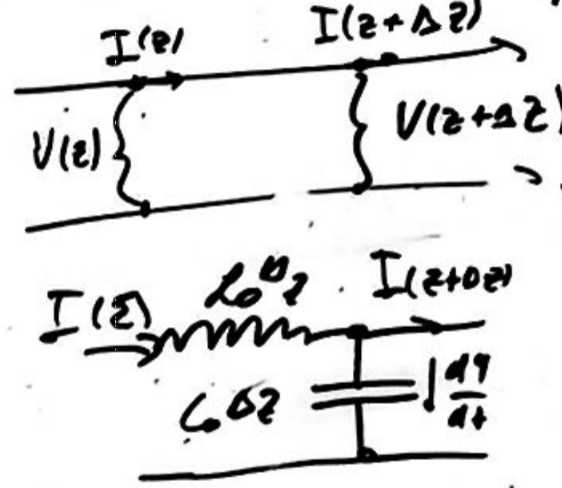
\includegraphics[width=0.25\textwidth]{img/2.png}
    %\caption{}
    %\label{fig:}
\end{figure}

\noindent
Из этих уравнений легко получить, что
\begin{equation}
    \left\{\begin{aligned}
        \frac{\partial U}{\partial z} &= - \frac{L_0}{c^2} \frac{d I}{d t} \\
        \frac{\partial I}{\partial z} &= - C_0 \frac{\partial U}{\partial t} 
    \end{aligned}\right.
    \hspace{0.5cm} \Rightarrow \hspace{0.5cm} 
    \boxed{
        \frac{\partial^2 U}{\partial t^2}  = \frac{c^2}{L_0 C_0} - \frac{\partial^2 V}{\partial z^2} 
    }.
\end{equation}
Решение аналогично будем искать в виде
\begin{equation}
    V = f_1 (z - vt) + f_2 (z + vt),
    \hspace{0.5cm} \Rightarrow \hspace{0.5cm} 
    v = \frac{c}{\sqrt{L_0 C_0}}.
\end{equation}
Кстати, если это всё посчитать для коаксиального кабеля, то
\begin{equation*}
    L_0 = 2 \mu \ln \frac{R_2}{R_1} , \hspace{0.5cm} 
    C_0 = \frac{\varepsilon}{2 \ln \frac{R_2}{R_1} },
    \hspace{0.5cm} \Rightarrow \hspace{0.5cm} 
    v = \frac{c}{\sqrt{\mu \varepsilon}}.
\end{equation*}


\subsubsection*{Коэффициент стоячей волны (standing wave ratio)}
Коэффициент стоячей волны -- отношение наибольшего значения амплитуды напряжённости электрического или магнитного поля стоячей волны в пучностях линии передачи к амплитуде в узлах.
КСВ является мерой согласования нагрузки (например, антенны) с линией передачи.

Наибольшее и наименьшее значения амплитуды соответсвенно равны
\begin{equation*}
    A_{\text{max}} = A_{\text{inc}} + A_{\text{ref}}, \hspace{0.5cm} 
    A_{\text{min}} = A_{\text{inc}} - A_{\text{ref}},
    \hspace{0.5cm} \Rightarrow \hspace{0.5cm} 
    \text{КСВ} = \frac{A_{\text{inc}} + A_{\text{ref}}}{A_{\text{inc}} - A_{\text{ref}}} = 
    \frac{1 + |\Gamma|}{1 - |\Gamma|},
\end{equation*}
где $|\Gamma|$ -- коэффициент отражения.

\subsubsection*{Согласованная нагрузка}
Рассмотрим длинную линию, пусть в цепи 
\begin{equation*}
    U = U_0 \cos \left(\omega_0 t - kz\right),  \hspace{0.5cm} 
    I = I_0 \cos \left(\omega_0 t - kz\right).
\end{equation*}
Сделаем следующий трюк. Возьмем, и продолжим линию до бесконечности, от которой, очевидно, ничего не отразится. Соотвественно нас интересует поиск эквивалентного импеданса системы. 
\begin{align*}
    U^* = U_0 \exp\left(i(\omega_0 t - kz)\right) &= U_0 e^{ikz} e^{-i\omega_0 t}, \\
    I^* = I_0 \exp\left(i(\omega_0 t - kz)\right) &= I_0 e^{ikz} e^{-i\omega_0 t}.
\end{align*}
Подставив эти выражения в волновое уравнение, и получим
\begin{equation*}
    ik U^* = i \omega_0 I^*,
    \hspace{0.5cm} 
    Z^* = U^* / I^* = \frac{\omega_0}{k},
    \hspace{0.5cm} \Rightarrow \hspace{0.5cm} 
    R = \frac{1}{c} \sqrt{\frac{L_0}{C_0}},
    \text{\ \ --- \ \ \textit{согласованная нагрузка}}.
\end{equation*}
То есть при наличии такого сопротивления на конце линии не будет никакого отражения. 



\newpage 

%%%%%%%%%%%%%%%%%%%%%%%%%%%%%%%%%%%%%%%%%%%%%%%%%%%%%%%%%%%%%%%%%%%%%%%%%%%%%%%%%%%
\setcounter{section}{5}
\addcontentsline{toc}{section}{Плазма}
%%%%%%%%%%%%%%%%%%%%%%%%%%%%%%%%%%%%%%%%%%%%%%%%%%%%%%%%%%%%%%%%%%%%%%%%%%%%%%%%%%%

\sbsnum{26}{Элементы физики плазмы}
\begin{to_def} 
    Замкнутое подмножество $M \subseteq \mathbb{R}^N$ называется \textit{вложенным многообразием размерности} $n$, если $\forall \ p \in M$ $\exists U_{\varepsilon}(p)$ и криволинейная система координат в ней, в которой включение $M \subset \mathbb{R}^N$ превращается в стандратное вложение $\mathbb{R}^n \subset \mathbb{R}^N$
    в пересечении с некоторой окрестностью нуля.
\end{to_def}

Яркий пример\footnote{
    Так, например, любая сфера в $\mathbb{R}^n$ является вложенным многообразием размерности $n-1$.
} -- работа с условными экстремумами. Если $M$ задаётся гладкими уравнениями $f_1 = \ldots = f_{N_n} = 0$ и дифференциалы этих уравнений линейно независимы в каждой точке $M$, то $M$ будет вложенным многообразием размерности $n$, так как определяющие его функции можно считать частью системы координат $y_{n+1}=f_1,\ldots,y_N=f_{N-n}$ в окрестности каждой точки $p \in M$, и $M$ в такой окрестности выглядит в точности как $\mathbb{R}^n \subset \mathbb{R}^N$ около нуля, а функции $y_1,\ldots,y_n$ задают систему координат в $M$, пересеченном с окрестностью $p$.


\begin{to_def} 
    Замкнутое подмножество $M \subseteq \mathbb{R}^N$ называется \textit{вложенным многообразием с краем\footnote{
        Край $\partial M$ многообразия с краем $M$ сам по себе является $(n-1)$-мерным многообразием без края.
    } размерности} $n$, если для $\forall \ p \in M \ \exists U_{\varepsilon}(p)$ и криволинейная система координат в ней, в которой включение $M \subseteq \mathbb{R}^N$ \textbf{либо} превращается в стандартное вложение $\mathbb{R}^n \subset \mathbb{R}^N$, \textbf{либо} превращается в стандартное вложение $(-\infty, 0] \times \mathbb{R}^{n-1} \subset \mathbb{R}^N$, пересеченное с окрестностью 0.
\end{to_def}


\begin{to_def} 
    Из определения $M$ понятно, что $\forall p \in M$  есть окрестность\footnote{
        Относительно открытое подмножество многообразия. 
    } в многообразие $M \cap U$ и отображение $\varphi \colon M \cap U \mapsto \mathbb{R}^n$, являющееся диффеоморфизмом между $M \cap U$ и $\varphi(M \cap U)$, которое называется \textit{координатной картой} многообразия $M$.
\end{to_def}


\begin{to_def} 
    Набор карт, районы действия которых в совокупности покрывают всё многообразие, называется \textit{атласом многообразия}. 
\end{to_def}

\newpage

%%%%%%%%%%%%%%%%%%%%%%%%%%%%%%%%%%%%%%%%%%%%%%%%%%%%%%%%%%%%%%%%%%%%%%%%%%%%%%%%%%%

%%%%%%%%%%%%%%%%%%%%%%%%%%%%%%%%%%%%%%%%%%%%%%%%%%%%%%%%%%%%%%%%%%%%%%%%%%%%%%%%%%%

